\section{Scelta del modello}
Si riportano i valori di $R^2$ e AIC dei quattro modelli.
\begin{table}[H]
	\centering
	\begin{tabular}{|c|c|c|}
		\hline
		\textbf{Modello} & \textbf{adjusted} \boldmath$R^2$ & \textbf{AIC} \\
		\hline
		1 &  0.77  & 514.69 \\
		2 & 0.87 & 460.76 \\
		3 & 0.77 & 514.11 \\
		4 & 0.89 & 448.27 \\
		\hline
	\end{tabular}
	\caption{Valori di $R^2$ e AIC per i quattro modelli}
\end{table}
Di seguito vengono mostrati i grafici diagnostici ottenuti sui quattro modelli.
\begin{figure}[H]
	\centering
	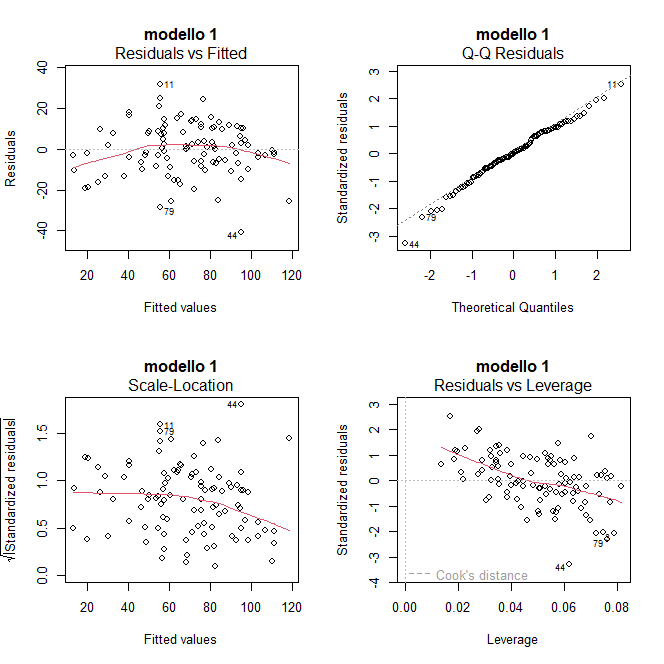
\includegraphics[width=0.95\linewidth]{../graphs/diagnostica/diagnostica_ridotto}
	\label{fig:diagnosticaridotto}
\end{figure}
\begin{figure}[H]
	\centering
	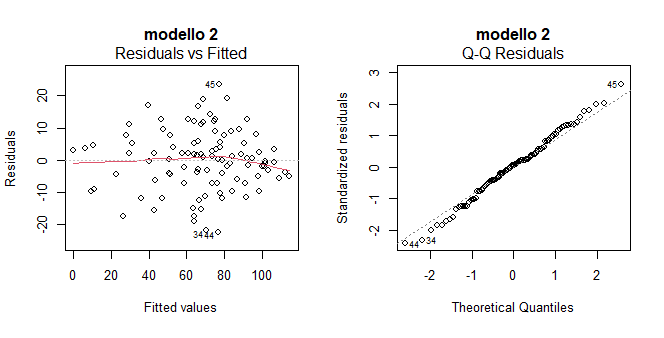
\includegraphics[width=0.95\linewidth]{../graphs/diagnostica/diagnostica_quadrato}
	\label{fig:diagnosticaridotto}
\end{figure}
\begin{figure}[H]
	\centering
	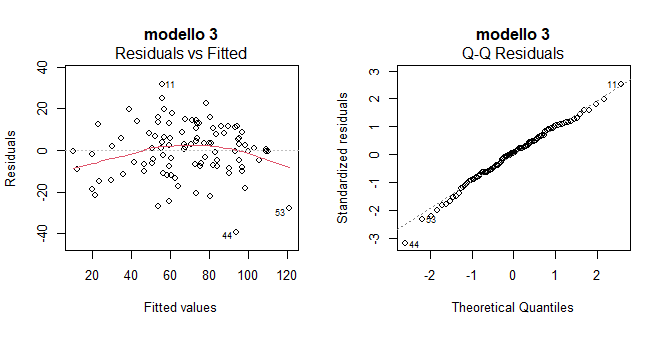
\includegraphics[width=0.95\linewidth]{../graphs/diagnostica/diagnostica_stepwise}
	\label{fig:diagnosticaridotto}
\end{figure}
\begin{figure}[H]
	\centering
	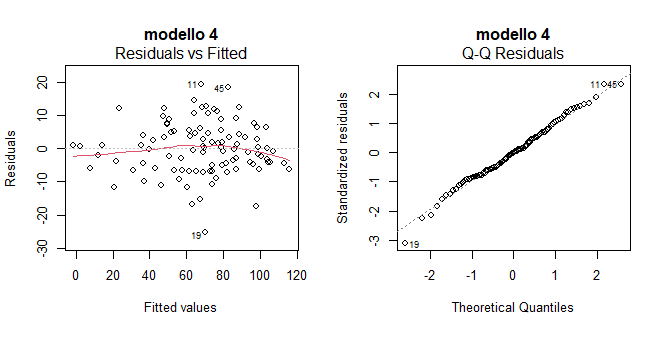
\includegraphics[width=0.95\linewidth]{../graphs/diagnostica/diagnostica_stepwise_iterations}
	\label{fig:diagnosticaridotto}
	\caption{Residuals vs Fitted e Q-Q Residuals dei quattro modelli.}
\end{figure}
Osservando i grafici 'Residuals vs Fitted' si nota che solo nei modelli 2 e 4, la linea rossa non presenta alcun pattern soddisfando in buona maniera l'ipotesi di linearità. Inoltre, sempre i modelli 2 e 4 nei grafici 'Q-Q Residuals' l'ipotesi di normalità sembra essere soddisfatta. 

Si osservi (dal grafico 'Scale-Location') che però su nessuno dei modelli considerati si può supporre che la varianza sia costante.

Infine comparando i valori di adjusted $R^2$ e AIC, il modello 4 sarebbe da preferire. Infatti, usando l'AIC, si sceglie il modello che ha valore minore; un valore maggiore di $R^2$ implica che il modello è in grado di interpretare meglio il fenomeno osservato.

A fronte dei dati ricavati si è stimato che il modello che meglio rappresenta il dataset fornito è il modello 4.


